% !TeX spellcheck = de_DE/GB

\chapter{Hardwarebeschreibung des Arduino}
\begin{figure}[htb]
	\begin{center}
		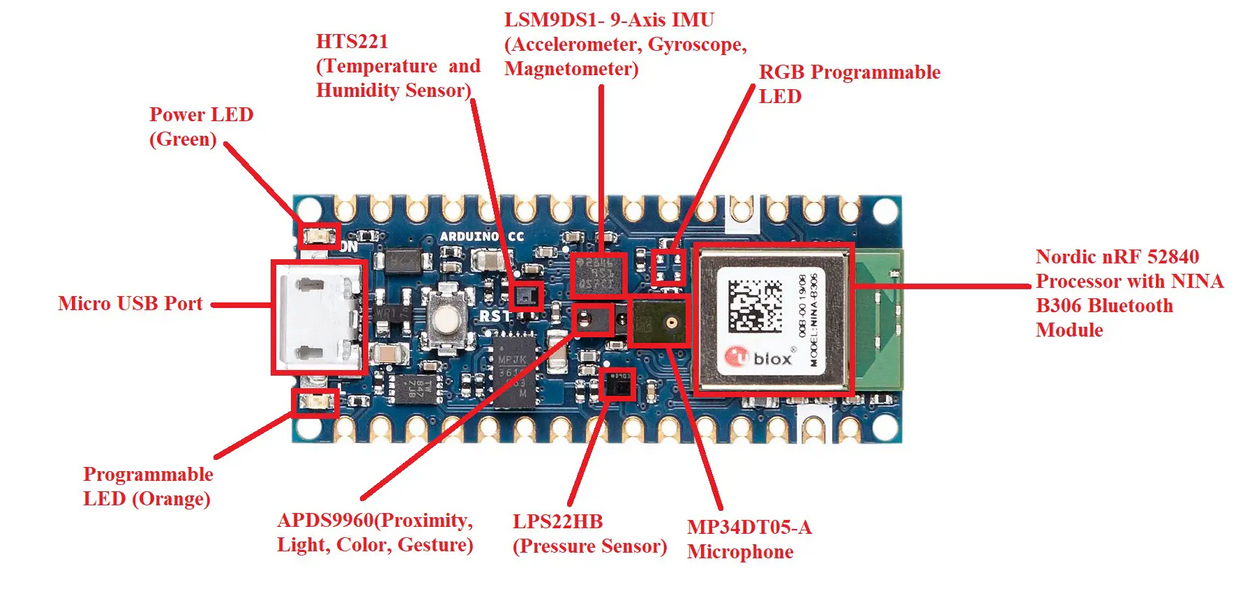
\includegraphics[width=\textwidth]{General/ArduinoBoard.png}
		\caption{Arduino Nano 33 BLE Sense}\cite{eTech.2021} \label{Arduino Nano 33 BLE Sense}
	\end{center}
\end{figure}
\section{Aufbau des Arduinos}
\cite{Ard.2024}
\\
Der Arduino Nano 33 Bluetooth Low Energie (BLE) Sense Lite ist ein Mikrocontroller basierend auf dem Nordic nRF52840-SoC (System-on-a-Chip). Trotz seiner kompakten Bauweise mit einer Größe von 45 x 18 mm verfügt es über mehrere verschiedene integrierte Sensoren, Aktoren und konnektive Schnittstellen (siehe \autoref{Arduino Nano 33 BLE Sense}). Zudem hat der Arduino-Prozessor einen 1 MB Flash-Speicher und 256 KB RAM. Bei dem Prozessor handelt es sich um einen Arm\textregistered Cortex-M4F Prozessorkern, welcher mit einer Taktrate von 64 MHz arbeitet und für Mikrocontroller Anwendungen optimiert ist. Dieser bietet eine gute Leistung bei geringen Stromverbrauch und ist auch für Echtzeitverarbeitungsaufgaben geeignet. Außerdem besitzt der Prozessor eine Floating Point Unit (FPU), wodurch sich Datenverarbeitungsoperationen effizient verarbeiten lassen.\cite{Arm}
Mithilfe einer integrierten Steckverbindung (engl. \glqq header \grqq) kann der Mikrocontroller direkt auf ein Board gesteckt werden. 

\section{Integrierte Sensorik}
Der Arduino Nano 33 BLE-Sense Lite verfügt über eine Vielzahl von integrierten Sensoren und Aktoren mit denen verschiedene Umwelteigenschaften detektiert werden können. Dazu gehören die in den folgenden Abschnitten beschriebenen Sensoren und Aktoren.
\subsection{9-Achs-IMU für die Bewegungserkennung (LSM9DS1)}
	Die Trägheitsmesseinheit LSM9DS1 ist ein System-in-Package, d.h. auf engsten Raum werden mehrere elektronische Komponenten oder Chips in einem Paket miteinander kombiniert.\cite{Wagner.2013} Die IMU verfügt über einen 3D-Linearbeschleunigungsmesser, ein 3D-Gyroskop und einen 3D-Magnetometer. Außerdem beinhaltet das System eine serielle I2C (Inter-Integrated-Circuit)-Bus Schnittstelle, die einen Standard und einen Fast Mode (100/400 kHz) bereitstellt, zudem eine serielle SPI-Standardschnittstelle. Der Sensor hat einen linearen Beschleunigungsmesser (Accelerometer) mit wählbarer Skala von ±2/±4/±8/±16 g, es misst die lineare Beschleunigung in drei Achsen (x, y, z) und ermöglicht die Erfassung von Änderungen der Geschwindigkeit und Position. Das Magnetfeld ist mit einer wählbaren Skala von ±4/±8/±12/±16 Gs ausgestattet, damit misst es das magnetische Feld in den drei Achsen und ermöglicht die Bestimmung der Ausrichtung relativ zur Erdmagnetfeldrichtung. Das 3D-Gyroskop ist mit wählbarem Skalenendwert: ±125/±250/±500/±1000/±2000 $\frac{Grad}{s}$ und ist dafür zuständig, die Winkelgeschwindigkeit bzw. Drehbewegung um die drei Achsen zu erfassen.\cite{STM1.2015}\cite{Ard.2024}
Mögliche Anwendungsbereiche sind zum Beispiel eine Bewegungssteuerungen (Drohnensteuerung, Robotik und industrielle Automatisierung), Schwingungsüberwachung und -kompensation, Antennen, Plattformen, optische Bild- und Objektivstabilisierung.  

\subsection{Näherungs-,Umgebungslicht-, Farb- und Gestensensor (APDS9960)}
	Hierbei handelt sich um einen sehr vielseitigen Sensor. Er dient zur Gestenerkennung, Farberkennung, Abstandsmessung und Umgebungslichtmessung. Die Gestenerkennung nutzt vier gerichtete Fotodioden, um reflektierte Infrarot-Energie (die von der integrierten LED stammt) zu erfassen, um die physischen Bewegungsinformationen (d.h. Geschwindigkeit, Richtung und Entfernung) in digitale Informationen zu übersetzen. Die Näherungserkennung ermöglicht die Messung der Entfernung durch die Erkennung der reflektierten Infrarot-Energie, (von der integrierten LED) mit Hilfe einer Fotodiode. Erkennungsereignisse sind interruptgesteuert und treten immer dann auf, wenn das Näherungsergebnis die oberen und/oder unteren Schwellenwerte überschreitet. Der Sensor verfügt zudem über Offset-Einstellregister, um den System-Offset zu kompensieren, der durch unerwünschte Infrarot-Energiereflexionen am Sensor entsteht. Die Infrarot-LED-Intensität ist werksseitig eingestellt, so dass eine Kalibrierung der Endgeräte aufgrund von Bauteilschwankungen nicht erforderlich ist. Die Farb- und Umgebungslichterkennung liefert Daten zur roten, grünen, blauen Farbspektrum und Daten zur klaren Lichtintensität. Jeder der Kanäle R, G, B, C hat einen UV- und Infrarot-Sperrfilter und einen speziellen Datenkonverter, der gleichzeitig 16-Bit-Daten erzeugt. Diese Architektur ermöglicht Anwendungen eine genaue Messung des Umgebungslichts zu messen und die Farbe zu erkennen, was es den Geräten wiederum ermöglicht, die Farbtemperatur zu berechnen und die Hintergrundbeleuchtung des Displays dementsprechend anzupassen.\cite{AT.2015}\cite{Ard.2024}
	
\subsection{Barometrischer Drucksensor (LPS22HB)}
	Der LPS22HB ist ein sehr kompakter Absolutdrucksensor, der auf dem piezoresistiven Prinzip basiert. Er fungiert als Barometer und verfügt über einen digitalen Ausgang. Zudem ist in diesem Drucksensor ein Temperatursensor integriert mit welchem Druckmessungen zusätzlich kompensiert werden können. Das Gerät besteht aus einem Sensorelement und einer Integrated-Circuit (IC)-Schnittstelle, die eine Kommunikation zwischen der Sensoreinheit und der Anwendung über Inter-Integrated Circuit (I2C) oder Serial Peripheral Interface (SPI) ermöglicht. Das Sensorelement erfasst den absoluten Druck und besteht aus einer speziell hergestellten, aufgehängten Membran. Der LPS22HB ist in einem vollständig vergossenem Land-Grid-Array-Gehäuse untergebracht, das kleine Löcher aufweist. Durch diese Öffnung gelangt der externe Druck auf das Sensorelement. Der Betrieb des Sensors ist über einen Temperaturbereich von -40 °C bis +85 °C gewährleistet. \cite{STM2.2017}\cite{Ard.2024}
	Anwendungsbereiche für diesen Sensor währen zum Beispiel: Wetterstationen, Höhenmesser, Luftdrucküberwachung in industriellen Prozessen oder tragbare smarte Geräte, wie Sportuhren oder Smartphones.
	
\subsection{Digitales Mikrophon (MP34DT05)}
Das MP34DT05-A ist ein kompaktes, stromsparendes, omnidirektionales, digitales
Mikrofon mit einem kapazitiven Sensorelement und einer IC-Schnittstelle.
Das Sensorelement, das in der Lage ist, akustische Wellen zu detektieren, wird mit
einem speziellen Silizium-Mikrobearbeitungsverfahren für die Herstellung von
Audiosensoren hergestellt. Die IC-Schnittstelle wird in einem speziellen Halbleiterherstellungsverfahren (CMOS-Verfahren) hergestellt, das die Entwicklung einer speziellen Schaltung ermöglicht, die ein digitales Signal im PDM (Pulsdichtenmodulation) -Format extern bereitstellen kann. Das Mikrofon hat einen Signal-Rausch-Abstand von 64 dB und eine Empfindlichkeit von -26 dBFS ±3 dB. Sein maximaler Schalldruckpegel liegt bei 122,5 dBSPL. Der MP34DT05-A ist in einem SMD-kompatiblen, EMI-geschirmten Top-Port-Gehäuse erhältlich und arbeitet zuverlässig über einen erweiterten Temperaturbereich von -40 °C bis +85 °C. Abmessungen des Gehäuses HCLGA-4 LD sind 3 x 4 x 1 (in mm). Anwendung findet das Modul Beispielsweise in mobilen Endgeräten, im Bereich der Spracherkennung sowie in Laptops und Notebooks.\cite{STM3.2021}\cite{Ard.2024}

\subsection{DC-DC-Wandler (MPM3610)}
Das MPM3610-Modul ist ein integriert Gleichspannungs- zu Gleichspannungs-Wandler. Dieser kann Eingangsspannungen von bis zu 21 V verarbeiten mit einem Wirkungsgrad von mindestens 65\% bei minimaler Last. Bei einer Eingangsspannung erhöht sich der Wirkungsgrad auf 85\%.\cite{Ard.2024}

\section{Beschreibung der Schnittstellen}
Der Arduino Nano 33 BLE-Sense Lite bietet eine Vielzahl von Schnittstellen, die das Board mit anderen Komponenten und Geräten einfach verbinden lassen. In diesem Abschnitt sind einige Details zu den wichtigsten Schnittstellen des Boards erläutert.
\begin{figure}[htb]
	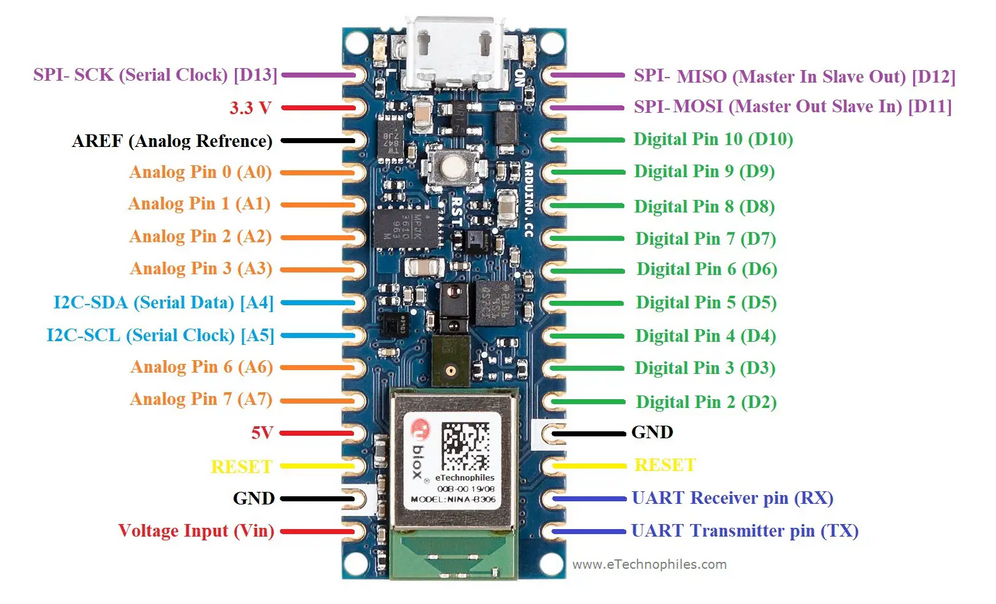
\includegraphics[width=14cm]{General/ArduinoPinBoard.png}
	\caption{Arduino Nano Pinboard} \label{Arduino Nano Pinbout}\begin{center}
		\cite{Arduino2023} %%% Bild später noch ändern und mit Tikz machen
	\end{center}
\end{figure}
\subsection{I2C}
Der Inter-Intergrated-Circuit (I2C) -Bus ermöglicht die Vernetzung von Mikrocontrollern, Sensoren, LED-Bildschirmen, Echtzeituhren und vielen anderen Bausteinen. Das Kommunikationsprotokoll basiert auf dem Master-Slave-Prinzip. Der Master initiiert und beendet die Kommunikation, stellt den Takt zur Synchronisation bereit und löst Kommunikationsprobleme. Jeder Slave hat eine eindeutige Adresse, mit einer Länge von 7 Bit und ermöglicht die Adressierung von bis zu 128 Slaves. Geräte mit unterschiedlichen Adresslängen können im selben Bus koexistieren. Bevor der Master Daten überträgt oder empfängt, muss er einen Slave mit einer vorher vereinbarten Adresse ansprechen.\cite{Meroth.2018}\cite{STM1.2015} Sind ihre Adressen in Übereinstimmung kann im nächsten Schritt ein einzelnes Bit gesendet werden, mit dem dann festgelegt wird, ob der Master Daten an dem Slave übertragen (Binär:1) oder auslesen möchte (Binär:0). Dieser Datenaustausch wird danach bestätigt, sodass weitere Daten ausgetauscht werden können. Zur Beendigung des Datenaustausches wird eine Stop-Signal gesendet.\cite{Gehrke.2022} In der minimalen Konfiguration werden Master und Slave über die bidirektionalen Busleitungen SDA und SCL verbunden, die über Pull-up-Widerstände an die Versorgungsspannung angeschlossen sind. Weitere Geräte können durch Verbindung ihrer SDA- und SCL-Anschlüsse mit den entsprechenden Busleitungen an den Bus angeschlossen werden.\cite{Meroth.2018} In diesem Projekt dient der Arduino als Master und ein zusätzlich angeschlossenes OLED-Bildschirm als Slave.

\subsection{USB:}
Das Board kann über einen Micro-Universal-Serial-Bus (Micro-USB) mit einem Computer verbunden werden, um es zu programmieren oder Daten zu übertragen. Die Datenübertragungsrate beträgt dabei 12 Mbit/s. Außerdem kann der Arduino über diesen USB-Port Strom beziehen.

\subsection{Bluetooth\textregistered 5}
Die Bluetooth-Verbindung kann als drahtloses Kommunikationsweg eingesetzt werden. Dieses Bluetooth-Protokoll hat eine Übertragungsrate von 2 Megabit pro Sekunde (Mbps) und eine Sendeleistung von +8 Dezibel Milliwatt (dBm). Die Empfindlichkeit beträgt dabei -95 dBm. Des weiteren verbraucht diese Verbindung im Sendebetrieb 4,8 mA und 4,6 mA im Empfangsbetrieb. Das Bluetooth Modul ist kompatibel mit mehreren Protokollen unter anderem mit dem \textit{Thread-Protokoll} und dem \textit{Zigbee-Protokoll}.\cite{Ard.2024}\cite{NrdSem3.2024}

\subsection{Weitere Kommunikationsschnittstellen}
\cite{Ard.2024}\cite{NrdSem3.2024}
\begin{itemize}
	\item \textbf{NFC-A-Tag:} Near Field Communication (NFC) ist eine zusätzliche Funktion zur drahtlosen Kommunikation über kurze Distanzen. Zudem besitzt der NFC-A-Tag die Funktionen sich in einen Bereitschaftsmodus versetzen zu lassen, dass durch ein NFC-fähiges Gerät dann initiiert werden kann. Außerdem unterstützt es \textit{touch-to-pair}, die Funktion ermöglicht eine Kopplung mit anderen NFC-fähigen Geräten durch Berührung.
	\item \textbf{Arm CryptoCell CC310 Security Subsystem:} Für die Durchführung kryptografischer Operationen und Sicherheitsaufgaben.\\ \cite{NrdSem.2024}
	\item \textbf{QSPI/SPI/TWI/$I^2$S/PDM/QDEC:} Verschiedene weitere serielle Kommunikationsschnittstellen, die für den Datenaustausch verwendet werden können.
	\item \textbf{EasyDMA:} Direkt Memory Access (DMA) ist für die Übertragung von Daten zwischen verschiedenen Speicherbereichen, ohne dabei die CPU zu belasten.\cite{Gehrke.2022}
	\item \textbf{Analog-Digital-Wandler (ADC):} Wandelt analoge Eingangsignale in digitale Daten um. Der Wandler hat eine Auflösung von 12 Bit und eine maximale Abtastrate von 200 Kilosamples pro Sekunde (ksps).
	\item \textbf{128-Bit-AES/ECB/CCM/AAR-Co-Prozessor:} Co-Prozessor für kryptografische Operationen, der auf dem Advanced Encryption Standard (AES) basiert. Dieser unterstützt verschiedene Betriebsmodi wie Electronic Codebook (ECB), Counter with CBC-MAC (CCM) und Automatic Address Recognition (AAR). \cite{NrdSem2.2024}
	\item \textbf{Quad-SPI-Schnittstelle 32 MHz:} SPI-Schnittstelle, die eine maximale Taktrate von 32 MHz unterstützt. Quad-SPI ermöglicht es, Daten schneller als die herkömmliches SPI zu übertragen, indem es vier Datenleitungen verwendet.\cite{NrdSem3.2023}
\end{itemize}

\subsection{Digitale Ein- und Ausgangspins}
Das Board verfügt über 14 digitale Ein- und Ausgangspins. Die digitalen Pins können nur zwei Zustände, nach dem Binär-System lesen: wenn ein Spannungssignal vorliegt und wenn kein Signal vorhanden ist (0 oder 1). Einige der Pins sind zudem zur Pulsweitenmodulation fähig (D3, D5, D6, D9, D10). Außerdem sind die digitalen Pins D11 und D12 als Master-Output-Slave-Input (MOSI) und als Master-Input-Slave-Output (MISO), in einer Serial-Peripheral-Interface (SPI) Kommunikation einsetzbar.\cite{Ard.2024}

\subsection{Analoge Eingangspins}
Die Platine hat zusätzlich 8 analogen Eingangspins (A0-A7) die wiederum als Analog-Digital-Wandler (ADC) verwendet werden können. Außerdem sind diese Pins als digitale Ein-/Ausgangspins konfigurierbar. Der Pin A0 kann zudem als Digital-Analog-Wandler (DAC) konfiguriert werden. Die beiden Pins A4 und A5 können außerdem für die I2C-Kommunikation verwendet werden. Dabei fungiert A4 als Datenleitung (SDA), während A5 als Taktleitung (SCL) fungiert.\cite{Ard.2024}

\subsection{Weitere Pins}
\begin{itemize}
	\item \textbf{+3,3 V}: Erzeugt interne Stromquelle im Gerät und wird als Referenzspannung verwendet.
	\item \textbf{VIN}: Stromversorgung
	\item \textbf{5V}: Gibt 5V an die externen Komponenten ab. 
	\item \textbf{RST-Pin}: Dient zum zurücksetzen des Arduinos.
	\item \textbf{AREF-Pin}: Liefert die Spannungsreferenz, die der Mikrocontroller zur Zeit verwendet.
	\\ \cite{Ard.2024}
\end{itemize}

\subsection{LED-Lampen}
\begin{itemize}
Im Arduino selbst sind 3 LED´s verbaut, die auch alle programmiert werden können. Diese sind vor allem für die Überprüfung der Sensorik oder Softwareprogrammen nützlich. Zu den LED-Lampen gehören: 
	\item Programmierbare Power-LED (grün): Zeigt an, dass das Arduino-Board eingeschaltet ist.
	\item Programmierbare LED (orange)
	\item Programmierbare RGB-LED
	\\ \cite{Ard.2024}
\end{itemize}

\section{Schaltplan}
fehlt noch...
%%%Bin noch unschlüssig, ob der Schaltplan hier oder später auftauchen soll.

\section{Hinweis Arduino 33 BLE Sense Lite \label{Hinweis Arduino 33 BLE Sense Lite}}
Der Arduino Nano 33 BLE Sense \underline{Lite} ist eine komprimierte Variante vom ursprünglichen Arduino Nano 33 BLE Sense, welcher zusätzlich noch über einen Temperatur- und Feuchtigkeitssensor verfügt. Der Lite hat stattdessen einen Drucksensor integriert, über welchem auch die Temperatur gemessen werden kann, jedoch nicht die Feuchtigkeit.\cite{PetrFilipi.2022}
\section{Bezugsquellen}
Als Bezugsquellen dienten vor allem Datenblätter der Hersteller. Die meisten Informationen konnten dem Datenblatt des Arduino entnommen werden, jedoch ist dazu anzumerken, dass sich dieses Datenblatt auf das Arduino 33 BLE Sense bezieht und nicht auf das Arduino 33 BLE Sense \emph{Lite}. Speziell zum \emph{Lite} gibt es jedoch kein Datenblatt, so wurden das Datenblatt vom Arduino 33 BLE Sense herangezogen. Dies stellt sonst kein Problem dar, da sich, wie in \ref{Hinweis Arduino 33 BLE Sense Lite} beschrieben, nur um eine komprimierte Version des Arduino 33 BLE Sense handelt.


